\chapter{Mediciones y resultados}
En este capítulo se presentan los resultados obtenidos del diseño del protocolo SPI, utilizado para controlar los convertidores D/A y A/D, así como la caracterización de las fotorresistencias. Además, se incluyen las imágenes obtenidas por medio de la matriz de fototransistores.


\section{Resultados de protocolo SPI}
A continuación, se presentan dos capturas de osciloscopio que muestran las mediciones realizadas al ADC. En las figuras siguientes, se pueden observar cuatro gráficos distintos: la señal número 1, en color azul, corresponde al comando de escritura utilizado para configurar el ADC; la señal número 2 representa la señal de reloj dclk generada; la señal 3 muestra el valor leído de uno de los canales del ADC; y, finalmente, la señal número 4 corresponde a la señal de chip select. Cabe destacar que las mediciones obtenidas coinciden con las especificaciones del datasheet del convertidor, validando el correcto funcionamiento del sistema. El proceso de lectura y escritura requieren un total de 24 ciclos de dclk para completarse.
\newpage
\subsection{ADC}
En esta imagen se puede observar que el ADC leyó un voltaje de 2V.

            \begin{figure}[hbtp]
                \centering
                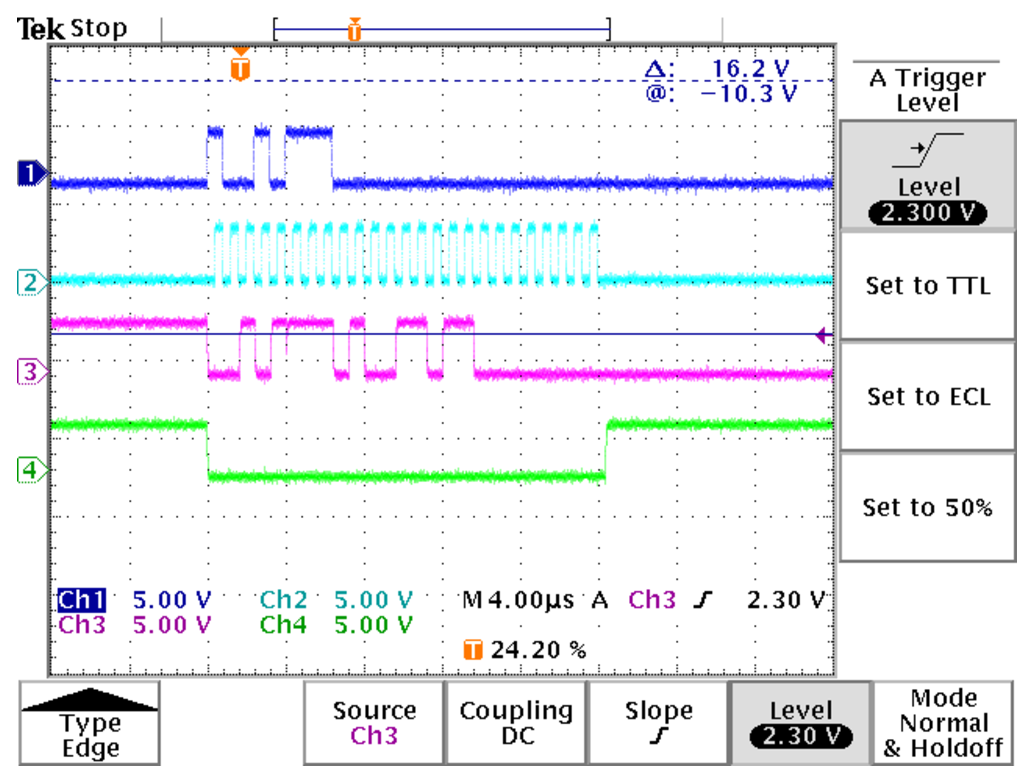
\includegraphics[width=0.6\textwidth]{ss_osc_adc_2v}
                \caption{Captura de osciloscopio de lectura y escritura de ADC.}
                \label{fig:ss_osc_adc_2v}
            \end{figure} 

En esta imagen se puede observar que la lectura corresponde a un voltaje de 3.3V
            \begin{figure}[hbtp]
                \centering
                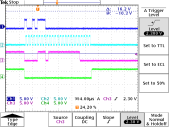
\includegraphics[width=0.6\textwidth]{ss_osc_adc_3v}
                \caption{Captura de osciloscopio de lectura y escritura de ADC.}
                \label{fig:ss_osc_adc_3v}
            \end{figure} 

\newpage     
\subsection{DAC}
Al igual que en el caso del ADC, se presentan las mediciones obtenidas por el osciloscopio para el DAC. En este caso, únicamente se muestra el proceso de escritura en el convertidor. La primera señal capturada corresponde a la señal de reloj del DAC (sck), que sincroniza la transferencia de datos. La segunda señal muestra el comando de 4 bits, seguido del valor de 12 bits que se desea escribir en el DAC. Finalmente, la tercera señal corresponde al chip select, que habilita el convertidor durante la operación de escritura. Estas mediciones permiten verificar el correcto funcionamiento del DAC, asegurando que los datos se transfieren de acuerdo con las especificaciones del dispositivo.


Esta imagen corresponde a una escritura de 2V.
            \begin{figure}[hbtp]
                \centering
                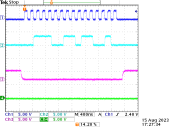
\includegraphics[width=0.6\textwidth]{ss_osc_dac_2v}
                \caption{Captura de osciloscopio de escritura de DAC.}
                \label{fig:ss_osc_dac_2v}
            \end{figure}
            
            
La siguiente imagen corresponde a una escritura de 3.3V           
            \begin{figure}[hbtp]
                \centering
                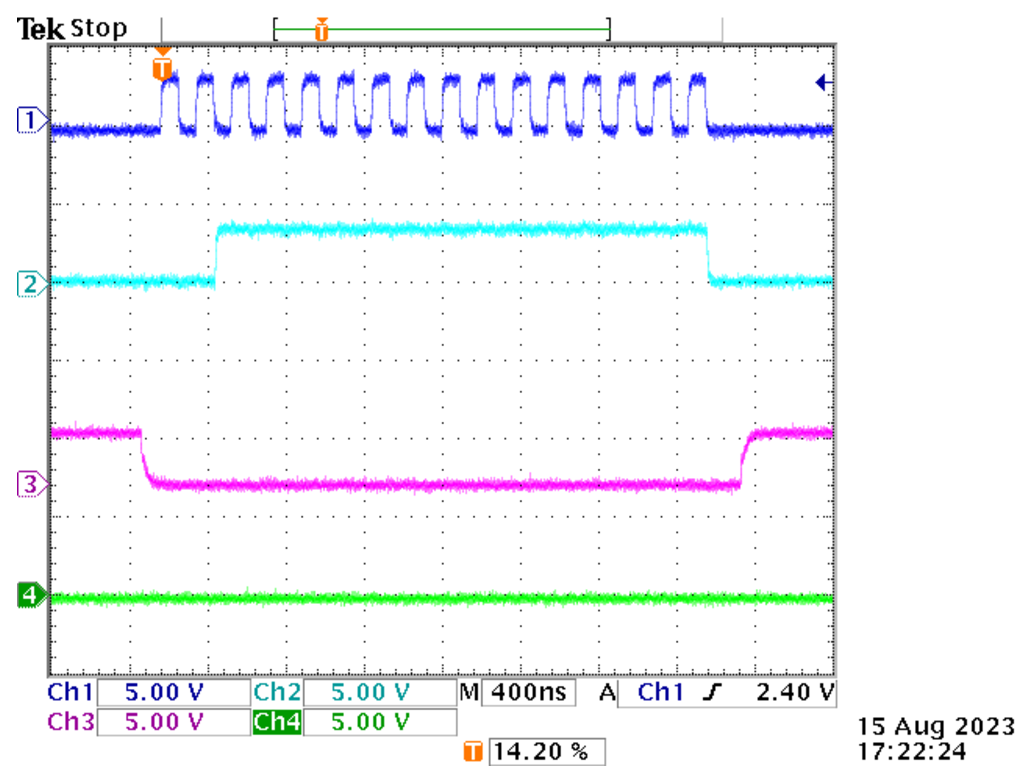
\includegraphics[width=0.6\textwidth]{ss_osc_dac_3v}
                \caption{Captura de osciloscopio de escritura de DAC.}
                \label{fig:ss_osc_dac_3v}
            \end{figure}   
            
\newpage                      
\section{Resultados de caracterización de resistencias}  
Al trabajar con la matriz de resistencias y al integrar los multiplexores en el sistema, se observó que el valor de voltaje recibido era menor de lo esperado. Este comportamiento anómalo llevó a sospechar que los multiplexores estaban introduciendo una resistencia adicional que afectaba las mediciones. Para investigar el impacto de esta resistencia en los resultados, se optó por medir la resistencia interna de los multiplexores. Esta medición permitió cuantificar el efecto de los multiplexores sobre los valores de voltaje obtenidos y ajustar el diseño para minimizar el impacto de esta resistencia en las lecturas.
            \begin{table}[htbp]
                \caption{Resistencia de multiplexores.}
                \begin{center}
                    \resizebox{0.9\linewidth}{!}{ 
                    \begin{NiceTabular}{| c | c | c | c | c | c |}
                        \CodeBefore
                        \Body
                        \hline
                        \textbf{$R_{test}$}  & \textbf{$V_{muxrows}$} & \textbf{$V_{muxcols}$} & \textbf{$i$} & \textbf{$R_{mux_{row}}$} & \textbf{$R_{mux_{col}}$}\\
                        \hline
                        1K$\Omega$   & 3.86e-2 V& 3.5e-2  V& 2.65e-4 A& 145.66 $\Omega$& 132$\Omega$\\
                        3.3K$\Omega$ & 3.43e-2 V& 3.1e-2  V& 2.21e-4 A& 155.2 $\Omega$& 140.27$\Omega$\\
                        5.6K$\Omega$ & 2.83e-2 V& 2.48e-2 V& 1.89e-4 A& 149.73 $\Omega$& 131.21$\Omega$\\
                        10K$\Omega$  & 2.25e-2 V& 2.11e-2 V& 1.49e-4 A& 151 $\Omega$& 141.6$\Omega$\\                            
                        \hline
                    \end{NiceTabular}
                    }
                \label{tab:Mux_res}
                \end{center}
            \end{table}

            \begin{figure}[hbtp]
                \centering
                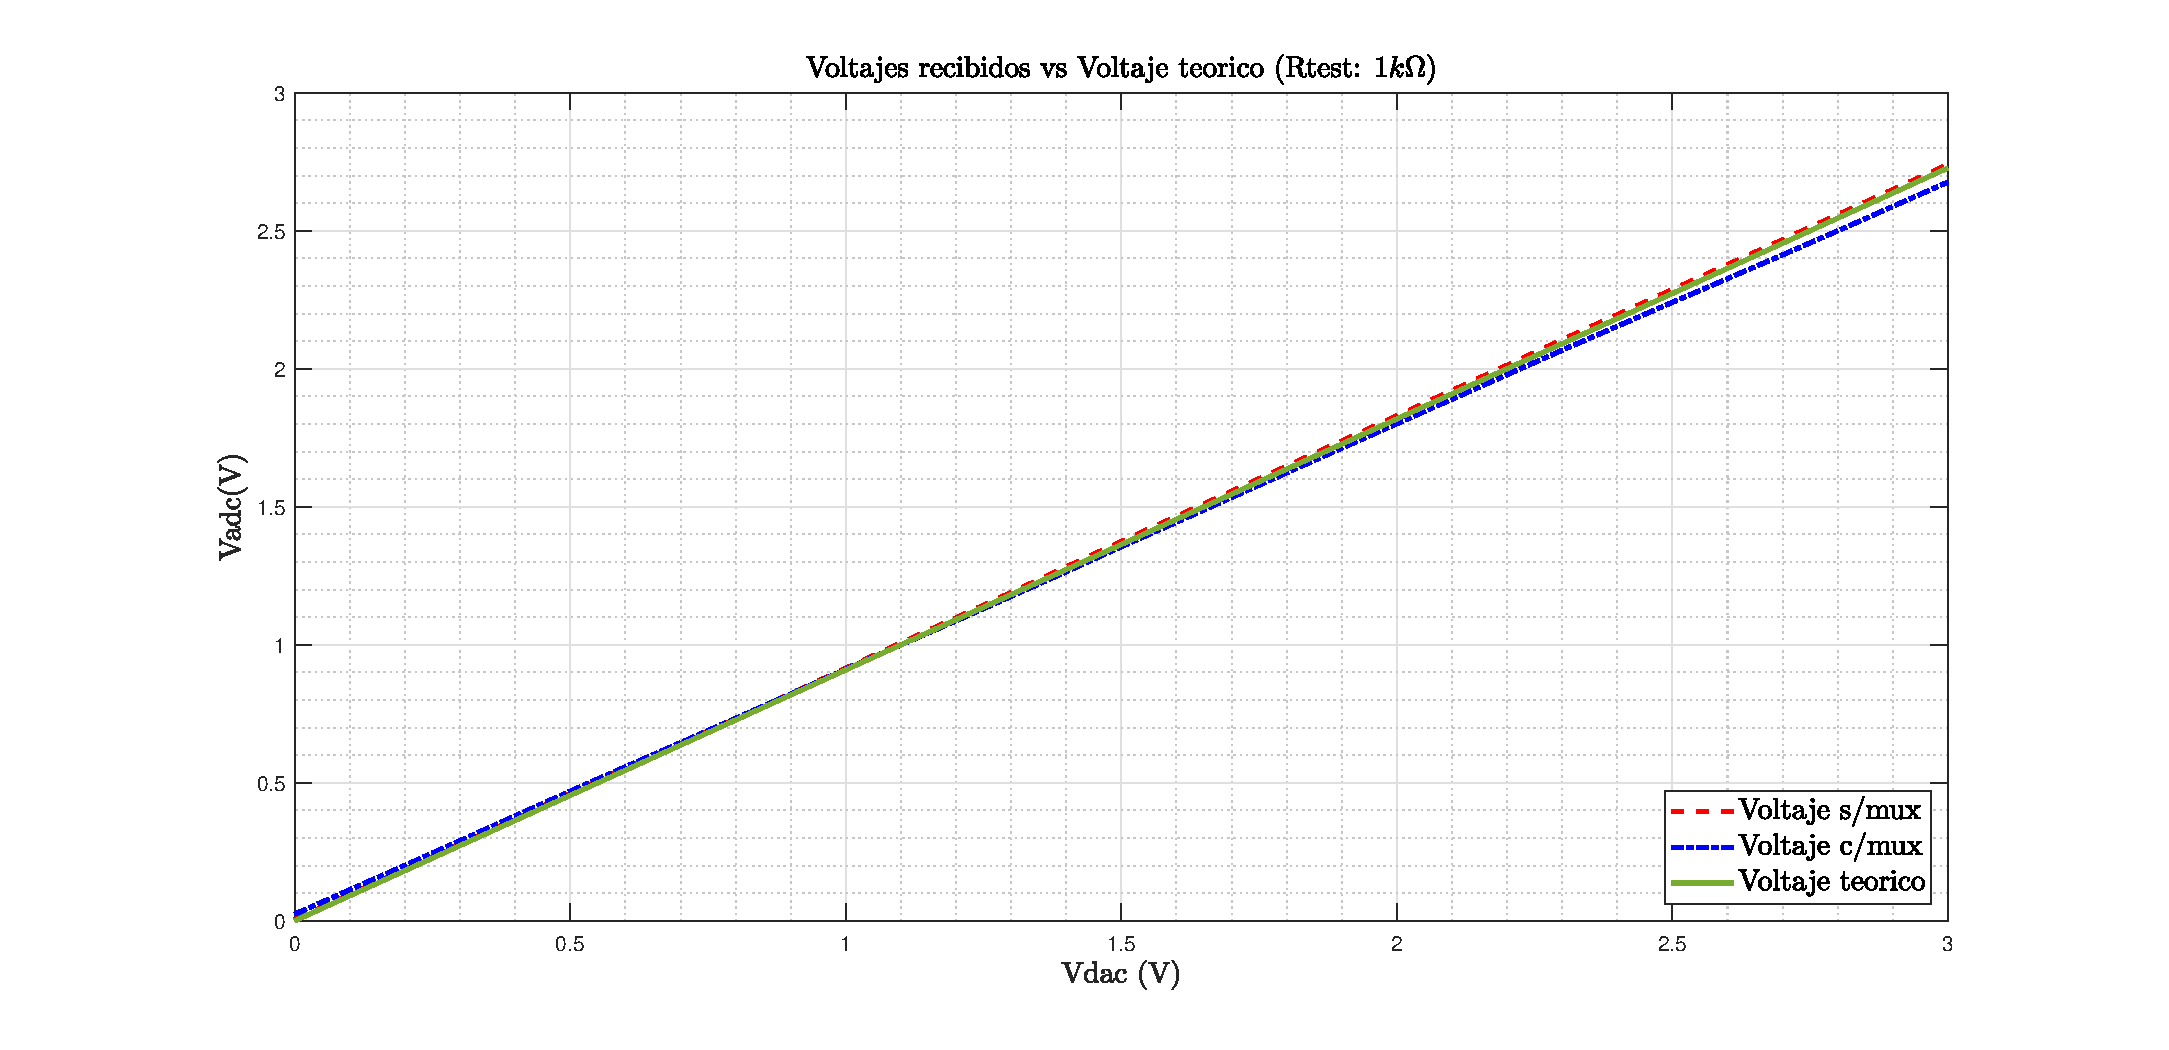
\includegraphics[width=1\textwidth]{01_1k}
                \caption{Influencia de resistencia de multiplexores.}
                \label{fig:01_1k}
            \end{figure}  
            
            \begin{figure}[hbtp]
                \centering
                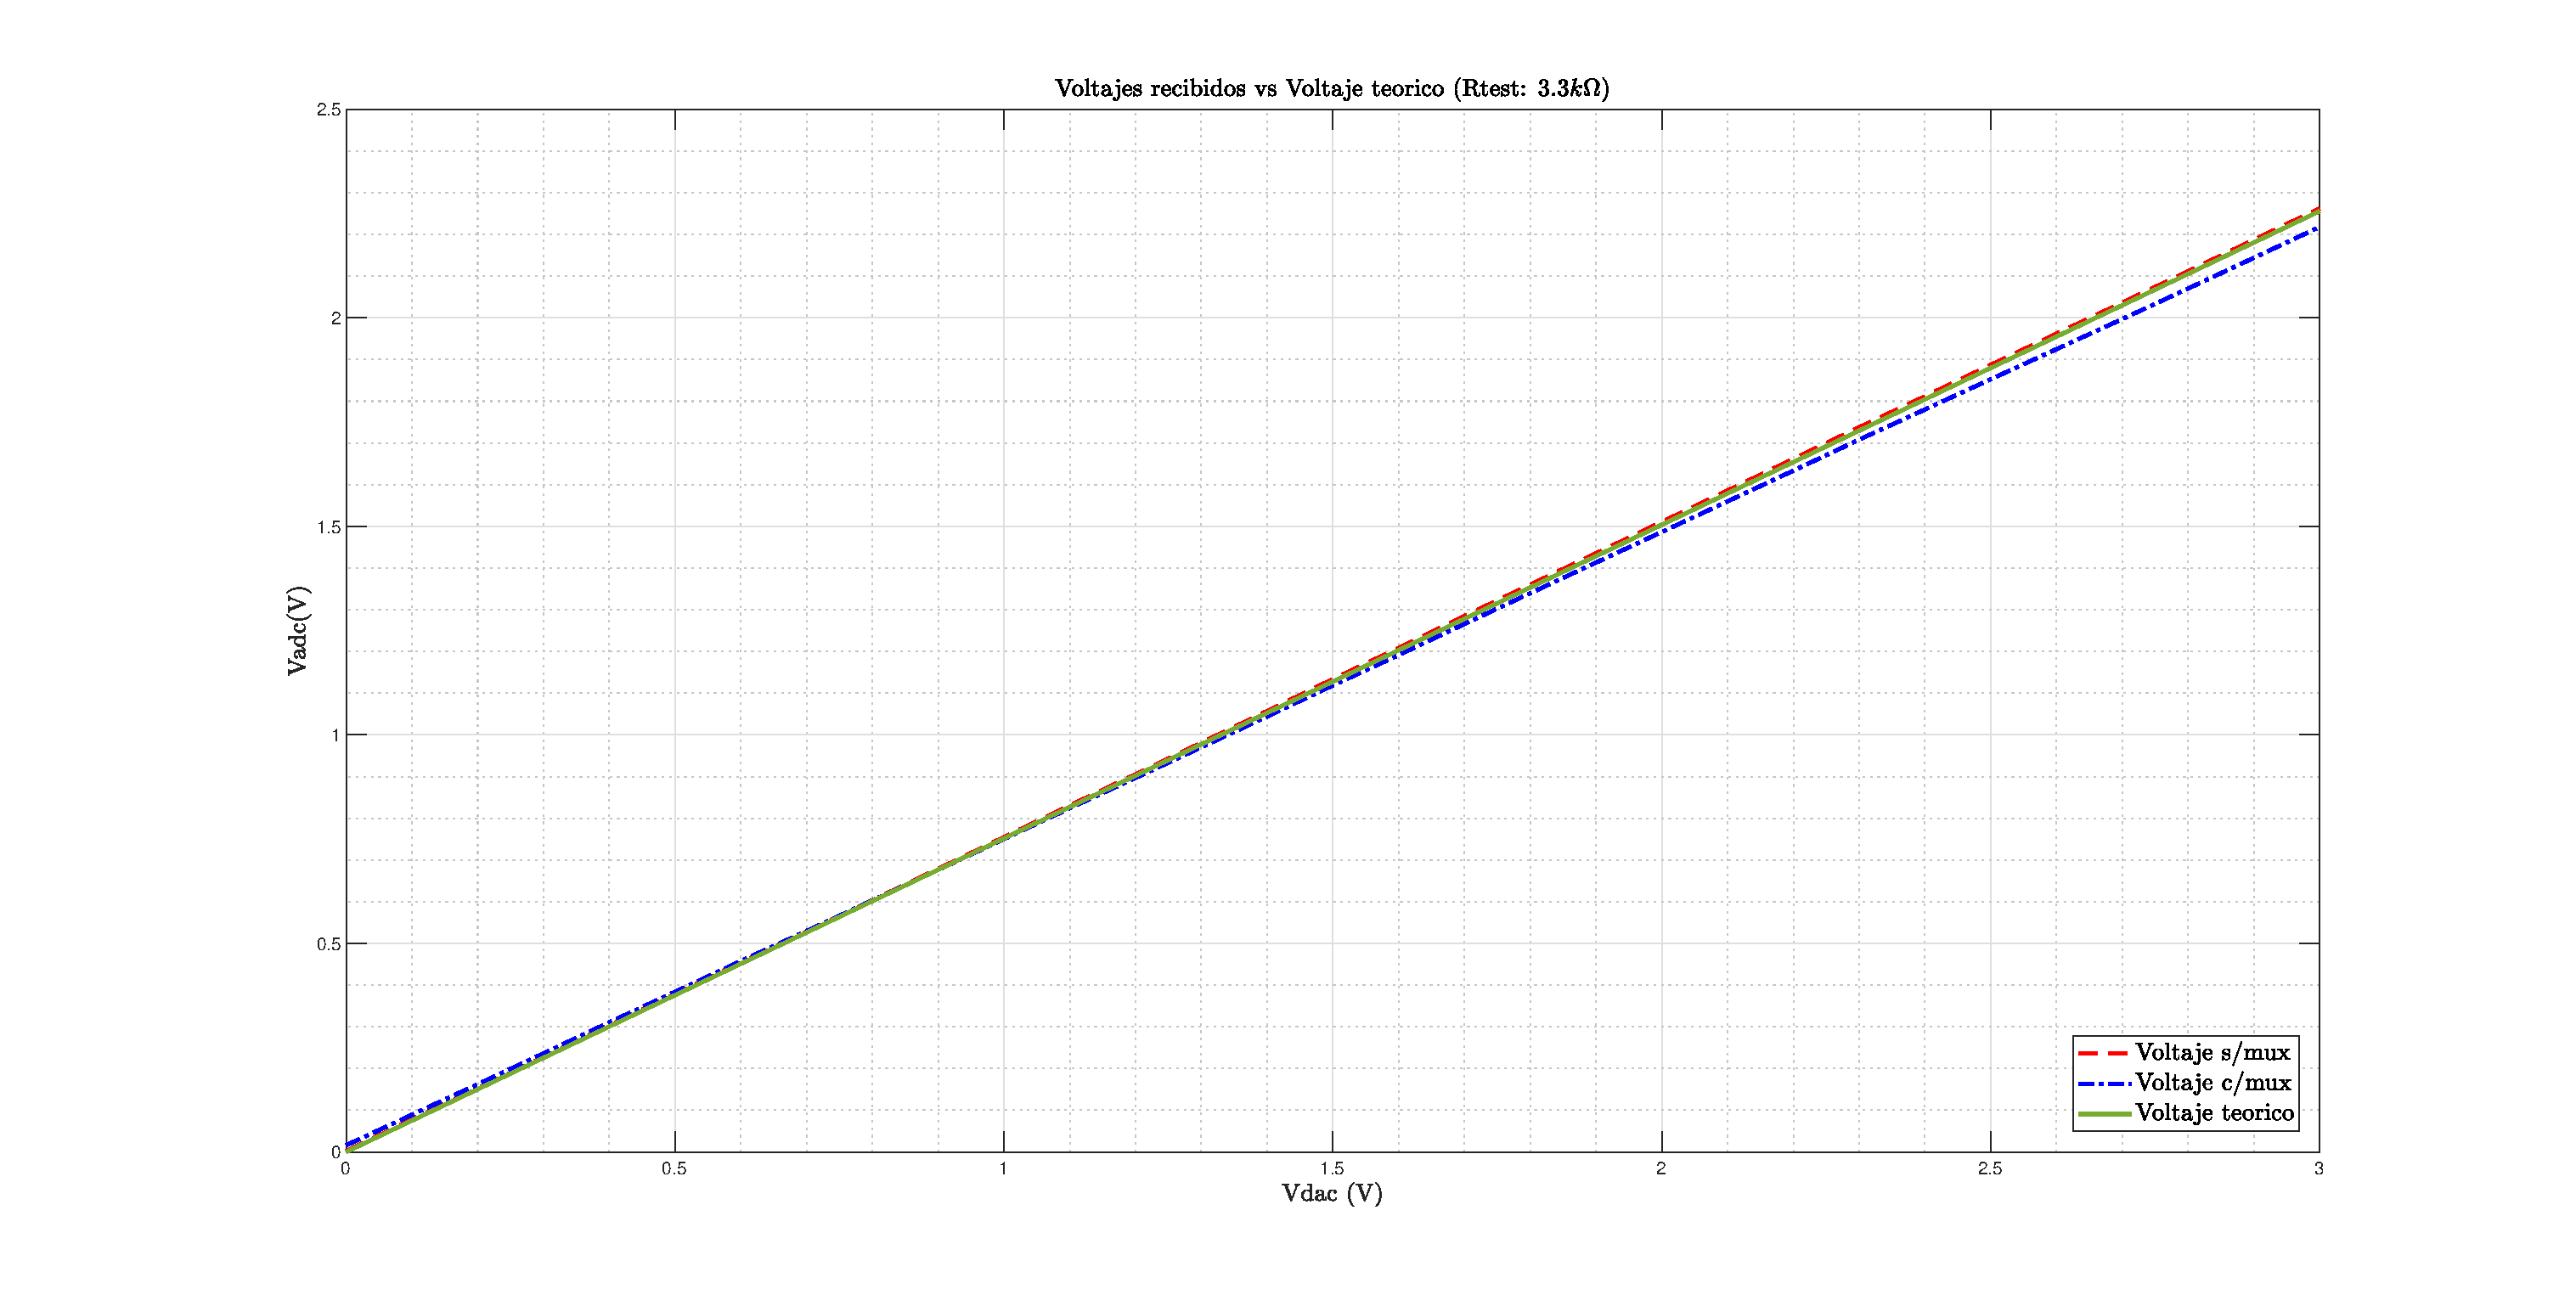
\includegraphics[width=1\textwidth]{02_3k3_new}
                \caption{Influencia de resistencia de multiplexores.}
                \label{fig:02_3k3_new}
            \end{figure}              
 
            \begin{figure}[hbtp]
                \centering
                \includegraphics[width=1\textwidth]{03_5k6_new}
                \caption{Influencia de resistencia de multiplexores.}
                \label{fig:03_5k6_new}
            \end{figure}   

            \begin{figure}[hbtp]
                \centering
                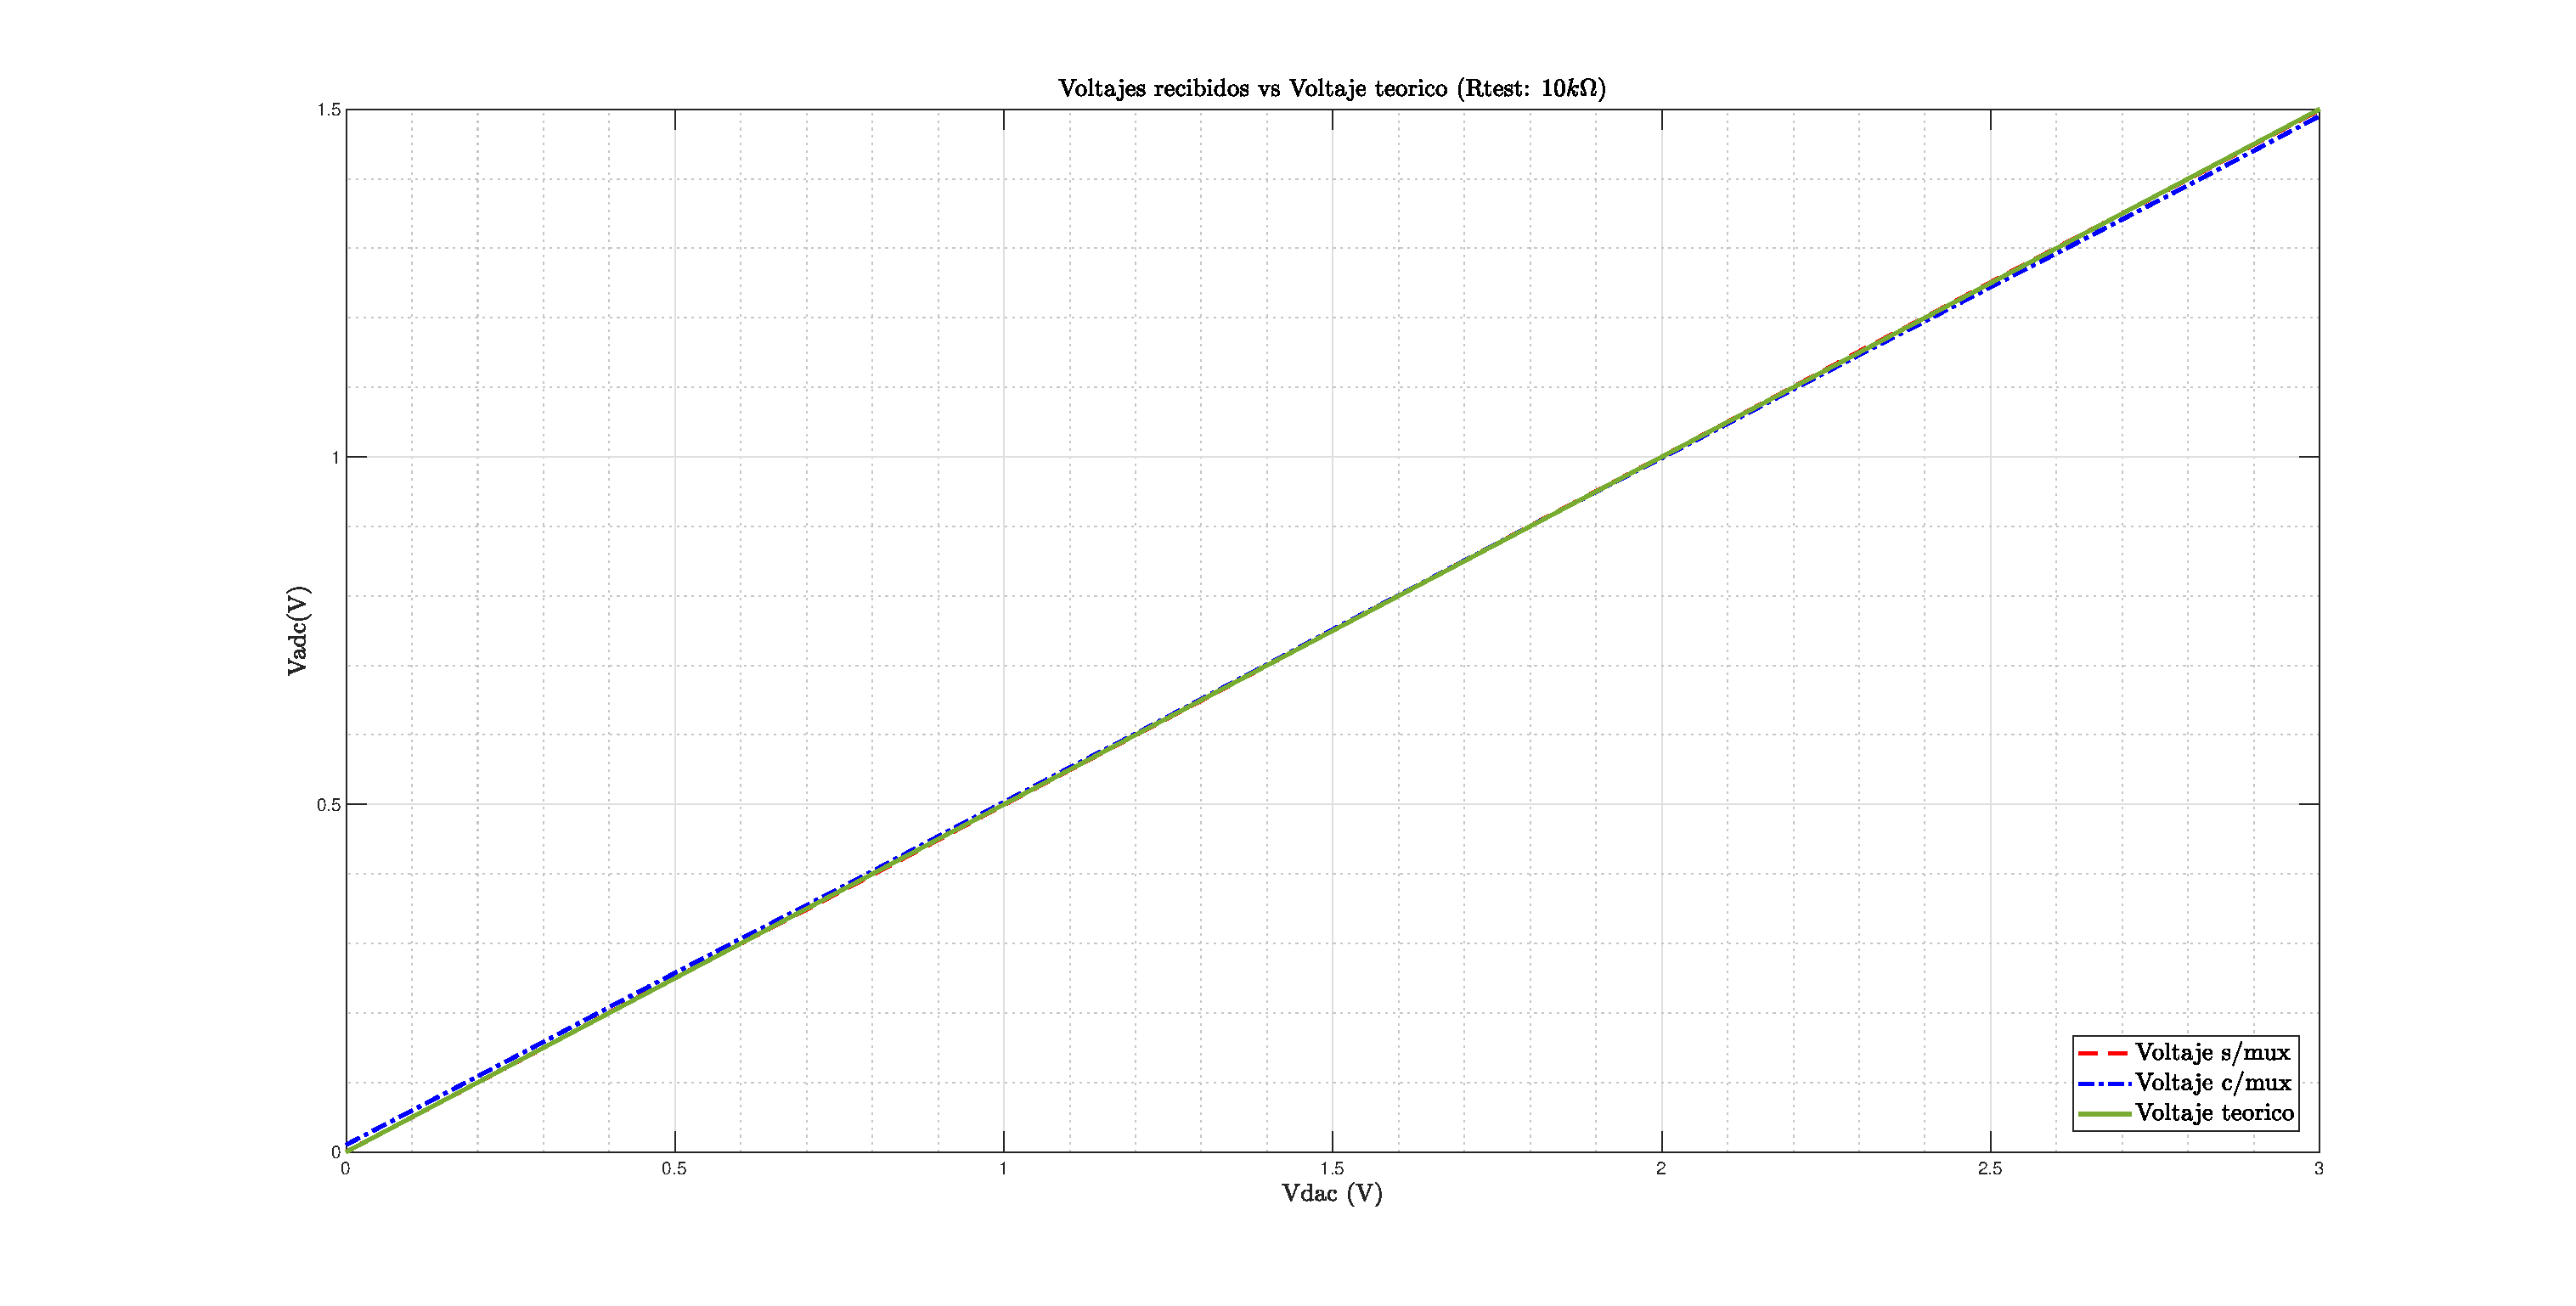
\includegraphics[width=1\textwidth]{04_10k_new}
                \caption{Influencia de resistencia de multiplexores.}
                \label{fig:04_10k_new}
            \end{figure}  
                
\newpage                      
\section{Resultados de caracterización de fotorresistencias}

            \begin{table}[htbp]
                \caption{Valor de fotorresistencias con diferentes duty cycles.}
                \begin{center}
                    \resizebox{0.6\linewidth}{!}{ 
                    \begin{NiceTabular}{| c | c | c |}
                        \CodeBefore
                        \Body
                        \hline
                        \textbf{$V_{Fuente}$}  & \textbf{Duty cycle ($\%$)} & \textbf{$R_{med} (K\Omega)$} \\
                        \hline
                        3 V     & 25  & 210 - 213.7\\
                                & 50  & 104 - 105.7\\
                                & 75  & 70 -71\\
                                & 100 & 53 - 54\\ \hline
                        3.3 V   & 25  & 29 - 31\\
                                & 50  & 16 - 17\\
                                & 75  & 11 - 12\\
                                & 100 & 8 - 9\\ \hline
                        3.5 V   & 25  & 6 - 7\\
                                & 50  & 3.6\\
                                & 75  & 2.6\\
                                & 100 & 2\\                             
                        \hline
                    \end{NiceTabular}
                    }
                \label{tab:Duty_cycle}
                \end{center}
            \end{table}


            \begin{figure}[hbtp]
                \centering
                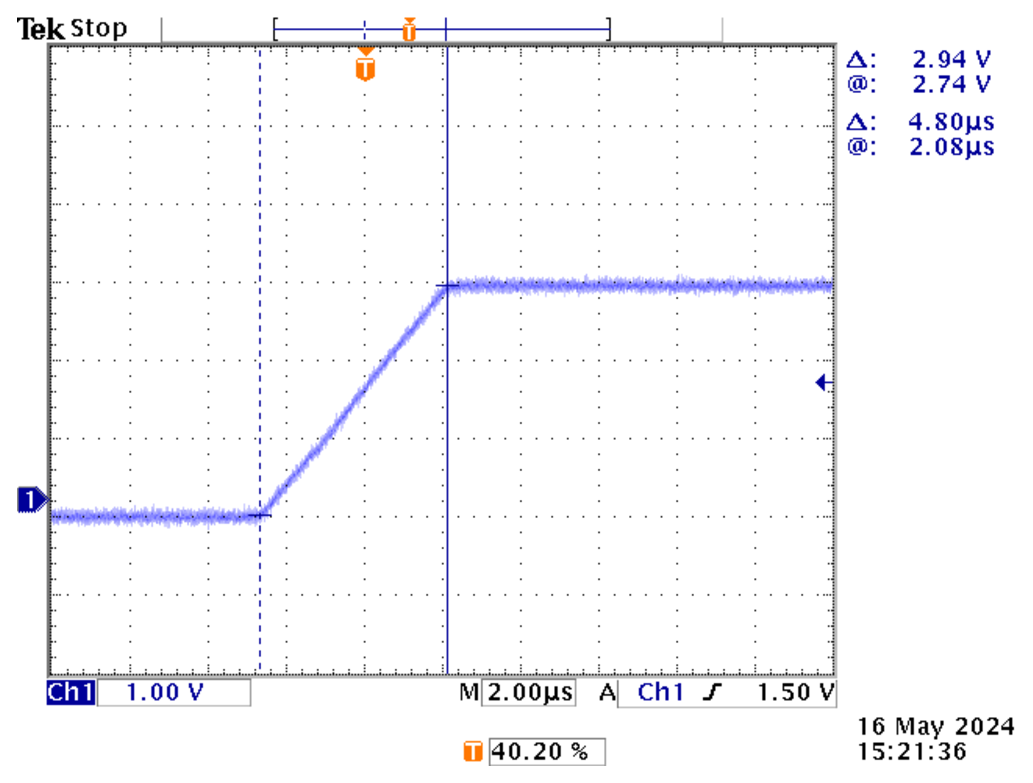
\includegraphics[width=0.6\textwidth]{settling_3v}
                \caption{Captura de osciloscopio de settling time.}
                \label{fig:settling_3v}
            \end{figure}
            
            \begin{figure}[hbtp]
                \centering
                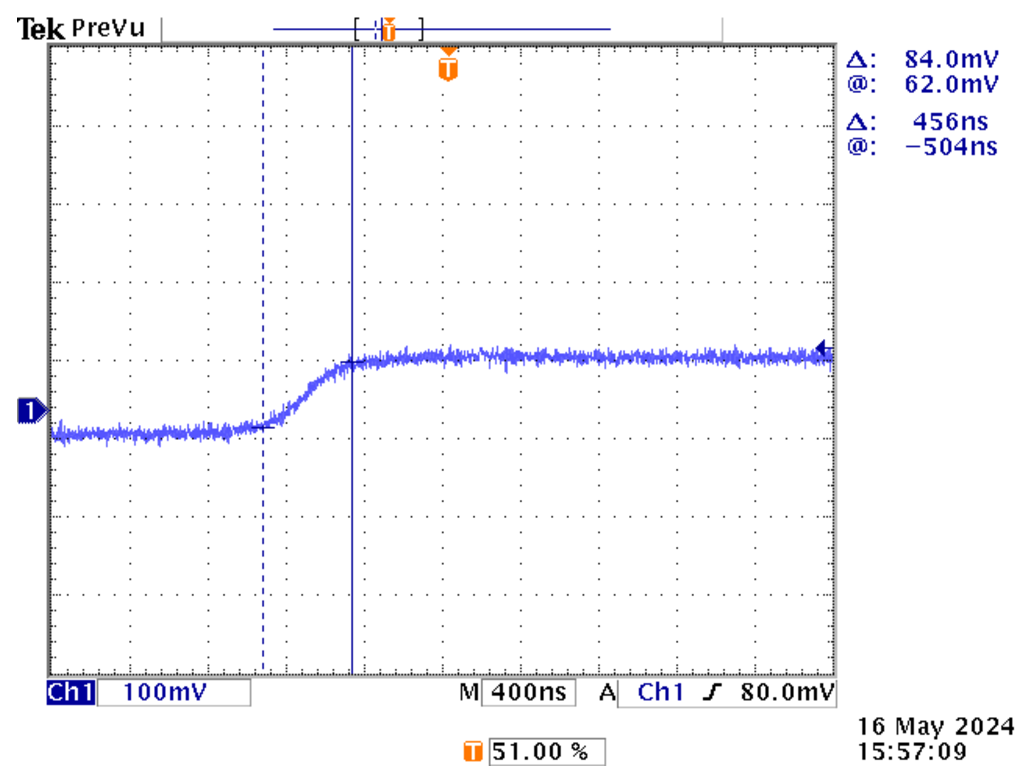
\includegraphics[width=0.6\textwidth]{settling_0v1}
                \caption{Captura de osciloscopio de settling time.}
                \label{fig:settling_0v1}
            \end{figure} 
            
            \begin{figure}[hbtp]
                \centering
                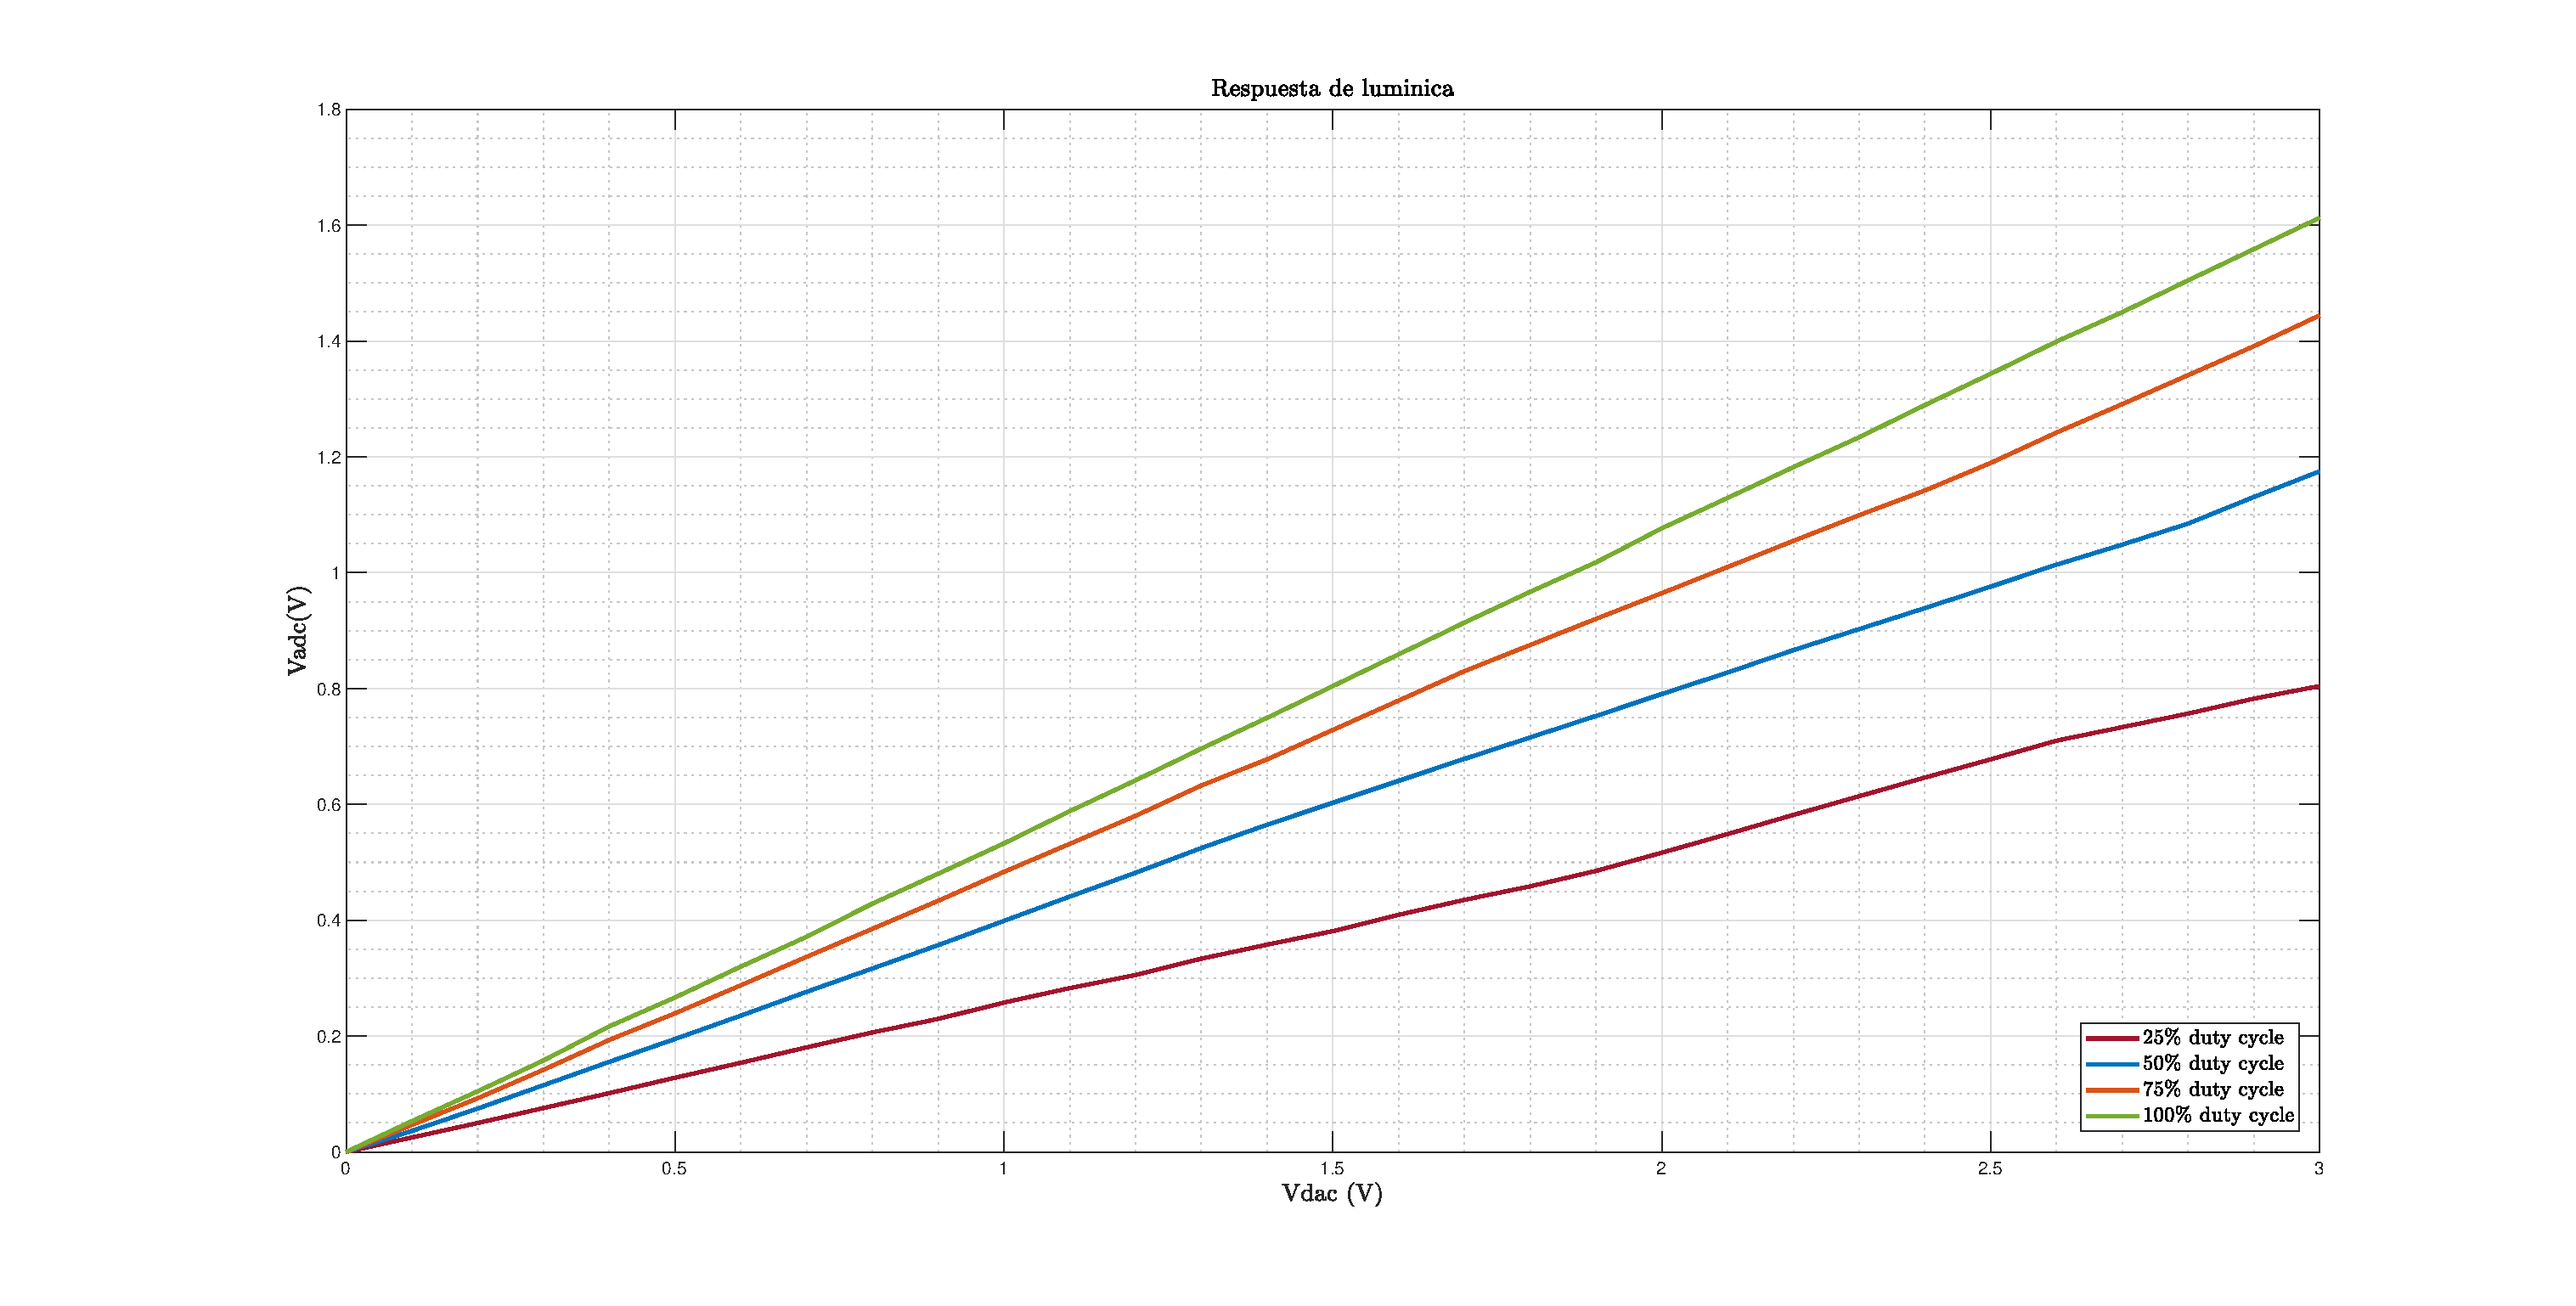
\includegraphics[width=1\textwidth]{respuesta_luminica}
                \caption{Respuesta lumínica.}
                \label{fig:respuesta_luminica}
            \end{figure}            
            
            
\newpage
\section{Imágenes obtenidas}

            \begin{figure}[hbtp]
                \centering
                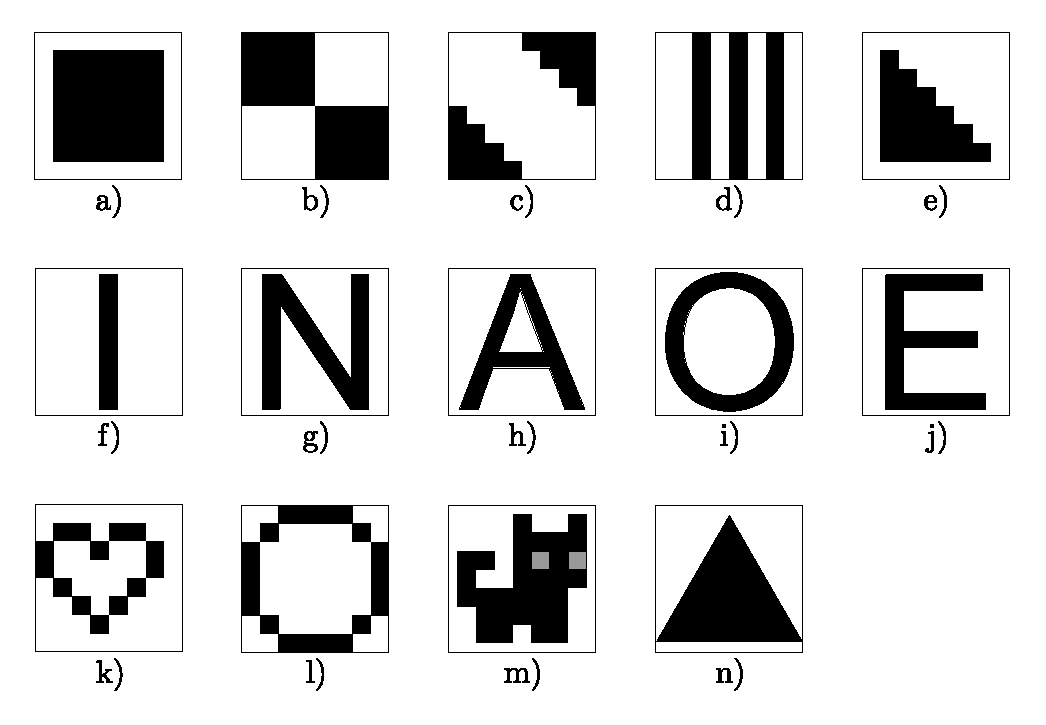
\includegraphics[width=0.8\textwidth]{mask_final}
                \caption{Máscaras aplicadas a matriz de fototransistores.}
                \label{fig:mask_final}
            \end{figure}  

            \begin{figure}[hbtp]
                \centering
                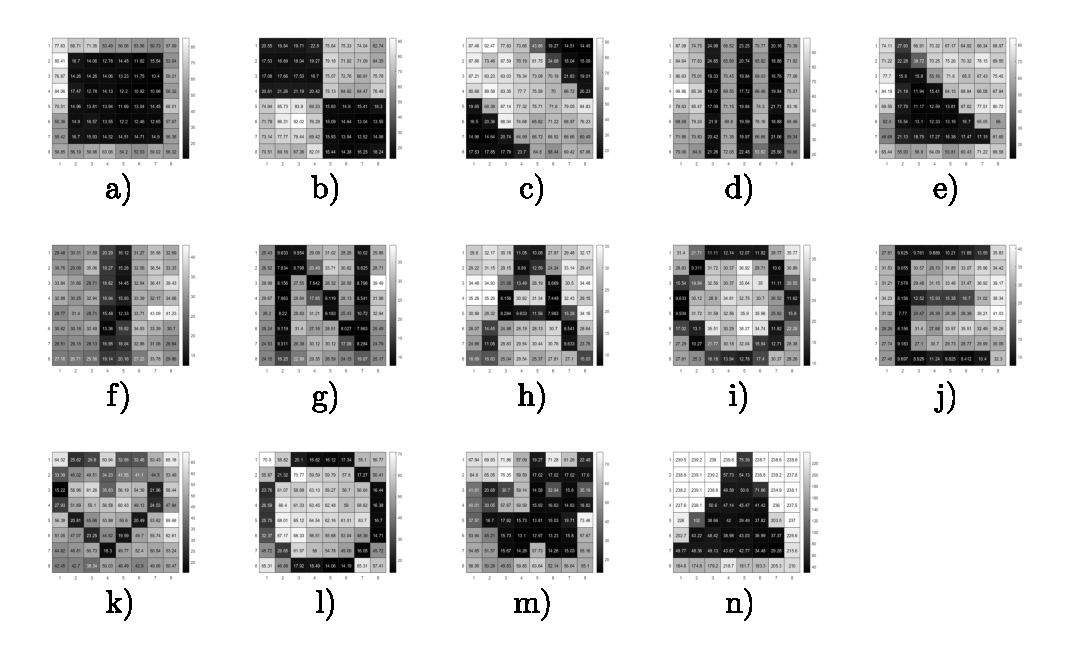
\includegraphics[width=0.8\textwidth]{result_mask}
                \caption{Resultados de las máscaras aplicadas a los fototransistores.}
                \label{fig:result_mask}
            \end{figure}
